% L12b Wolfram market schematic (November 2026). One step of the model as a loop:
% the traders' intentions go to the dealer as a net trade, the dealer quotes a
% price, the price moves the technical traders' band, and the band sets the edge
% intentions. Interior traders update from their four neighbors and their rule
% table (the rule-switch figure shows that lookup). Schematic only, no results.
%
% Style: same as Fig-L12b-RuleSwitch (pdflatex standalone, Computer Modern,
% pastel tiles with paper-palette borders). Teal marks the technical traders.
\documentclass[border=4pt]{standalone}
\usepackage{tikz}
\usepackage{amsmath,amssymb}
\usetikzlibrary{arrows.meta,calc}
\definecolor{buyblue}{HTML}{0072B2}
\definecolor{holdgray}{HTML}{AAAAAA}
\definecolor{sellorange}{HTML}{D55E00}
\definecolor{tech}{HTML}{0E7C86}
\definecolor{ink}{HTML}{252525}

\begin{document}
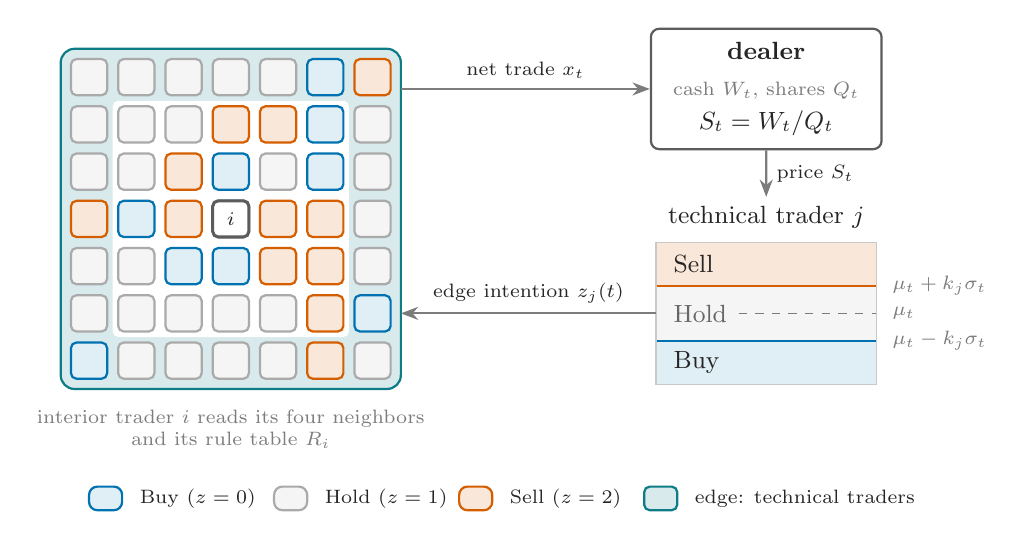
\begin{tikzpicture}[
  x=1cm,y=1cm,
  every node/.style={font=\small,text=ink},
  note/.style={font=\scriptsize,text=ink!60},
  box/.style={rectangle,rounded corners=3pt,thick,inner sep=2pt,align=center},
  buy/.style={box,draw=buyblue,fill=buyblue!12},
  hold/.style={box,draw=holdgray,fill=holdgray!12,text=ink!70},
  sell/.style={box,draw=sellorange,fill=sellorange!15},
  me/.style={box,draw=ink!75,fill=white,line width=1.1pt},
  cell/.style={minimum width=.46cm,minimum height=.46cm,rounded corners=2pt,inner sep=0pt},
  arr/.style={-{Stealth[length=2.2mm]},thick,ink!60},
]
% ---- the grid: 7 x 7, edge ring = technical traders ----
\def\gp{.6}
\fill[tech!16,rounded corners=5pt] (-.36,-.36) rectangle (6*\gp+.36,6*\gp+.36);
\draw[tech,thick,rounded corners=5pt] (-.36,-.36) rectangle (6*\gp+.36,6*\gp+.36);
\fill[white,rounded corners=2pt] (.3,.3) rectangle (6*\gp-.3,6*\gp-.3);
\foreach \r in {0,...,6} {
  \foreach \c in {0,...,6} {
    \pgfmathtruncatemacro{\edge}{(\r==0)||(\r==6)||(\c==0)||(\c==6)}
    \ifnum\edge=1
      \pgfmathtruncatemacro{\s}{mod(5*\r+3*\c+2*\r*\c,7)}
      \ifcase\s \def\st{buy}\or \def\st{sell}\else \def\st{hold}\fi
    \else
      \pgfmathtruncatemacro{\s}{mod(3*\r*\r+5*\c*\c+7*\r*\c+11*\r+13*\c+2,9)}
      \ifnum\s<3 \def\st{buy}\else\ifnum\s<6 \def\st{hold}\else \def\st{sell}\fi\fi
    \fi
    \node[\st,cell] (g\r\c) at (\c*\gp,\r*\gp) {};
  }
}
% trader i and its four neighbors
\node[me,cell,font=\scriptsize] at (3*\gp,3*\gp) {$i$};

% ---- dealer ----
\node[box,draw=ink!75,fill=white,inner xsep=8pt,inner ysep=5pt] (dealer) at (8.6,3.45)
  {\textbf{dealer}\\[2pt]{\scriptsize\color{ink!60}cash $W_{t}$, shares $Q_{t}$}\\[1pt]$S_{t}=W_{t}/Q_{t}$};

% ---- technical trader's band ----
\def\bx{7.2}\def\bw{2.8}\def\by{-.3}
\fill[buyblue!12]    (\bx,\by)     rectangle (\bx+\bw,\by+.55);
\fill[holdgray!12]   (\bx,\by+.55) rectangle (\bx+\bw,\by+1.25);
\fill[sellorange!15] (\bx,\by+1.25) rectangle (\bx+\bw,\by+1.8);
\draw[buyblue,thick]     (\bx,\by+.55) -- (\bx+\bw,\by+.55);
\draw[sellorange,thick]  (\bx,\by+1.25) -- (\bx+\bw,\by+1.25);
\draw[ink!60,dashed]     (\bx+1.05,\by+.9) -- (\bx+\bw,\by+.9);
\node[anchor=west] at (\bx+.1,\by+1.525) {Sell};
\node[anchor=west,text=ink!70] at (\bx+.1,\by+.9) {Hold};
\node[anchor=west] at (\bx+.1,\by+.275) {Buy};
\node[note,anchor=west] at (\bx+\bw+.08,\by+1.25) {$\mu_{t}+k_{j}\sigma_{t}$};
\node[note,anchor=west] at (\bx+\bw+.08,\by+.9) {$\mu_{t}$};
\node[note,anchor=west] at (\bx+\bw+.08,\by+.55) {$\mu_{t}-k_{j}\sigma_{t}$};
\node[anchor=south] (bandtitle) at (\bx+.5*\bw,\by+1.85) {technical trader $j$};
\draw[ink!25] (\bx,\by) rectangle (\bx+\bw,\by+1.8);

% ---- the loop ----
\draw[arr] (6*\gp+.36,3.45) -- (dealer.west) node[midway,above,note,text=ink] {net trade $x_{t}$};
\draw[arr] (dealer.south) -- (bandtitle.north) node[midway,right,note,text=ink] {price $S_{t}$};
\draw[arr] (\bx,\by+.9) -- (6*\gp+.36,\by+.9) node[midway,above,note,text=ink] {edge intention $z_{j}(t)$};

% ---- notes under the grid ----
\node[note,anchor=north,align=center] at (3*\gp,-.5) {interior trader $i$ reads its four neighbors\\and its rule table $R_{i}$};

% ---- legend ----
\foreach \xx/\st/\label in {0/buy/Buy ($z=0$),2.35/hold/Hold ($z=1$),4.7/sell/Sell ($z=2$)} {
  \node[\st,minimum width=.42cm,minimum height=.3cm] at (\xx+.21,-1.75) {};
  \node[note,text=ink,anchor=west] at (\xx+.52,-1.75) {\label};
}
\fill[tech!16,rounded corners=2pt] (7.05,-1.9) rectangle (7.47,-1.6);
\draw[tech,thick,rounded corners=2pt] (7.05,-1.9) rectangle (7.47,-1.6);
\node[note,text=ink,anchor=west] at (7.57,-1.75) {edge: technical traders};
\end{tikzpicture}
\end{document}
